\documentclass[11pt,reqno]{amsart}

\usepackage{amsmath,amssymb,amsthm,amsfonts,mathtools}
\usepackage{tikz}
\usepackage[hidelinks]{hyperref}
\usepackage[a4paper,margin=1in]{geometry}
\usepackage{caption}
\captionsetup[table]{position=below,skip=12pt}

% Tolerate long, unbreakable \texttt{...} Lean identifiers without
% producing visible right-margin overruns.
\tolerance=2000
\emergencystretch=5em
\hbadness=2000   % don't warn about minor underfull \hbox
\hyphenpenalty=50

\theoremstyle{plain}
\newtheorem{theorem}{Theorem}[section]
\newtheorem{lemma}[theorem]{Lemma}
\newtheorem{corollary}[theorem]{Corollary}
\newtheorem{proposition}[theorem]{Proposition}

\theoremstyle{definition}
\newtheorem{definition}[theorem]{Definition}

\theoremstyle{remark}
\newtheorem{remark}[theorem]{Remark}
\newtheorem{example}[theorem]{Example}

\title[Period Formulas for Rational Cut-and-Project Projections]{%
  Period Formulas for Rational Cut-and-Project Strip Projections:
  Multiset and Set Cases}

\author{Dirk Kunert}
\address{Independent Researcher}
\email{dirk.kunert@gmail.com}

\subjclass[2020]{Primary 52C23; Secondary 11B25, 37B10, 68V20, 11A07}
\keywords{cut-and-project sets, projected multisets, gap sequences,
period length, set-valued period, multiplicity conventions,
rational slope, residue classes, lattice projection,
Lean~4 formalization}

\date{\today}

\begin{document}

\begin{abstract}
Consider the one-dimensional cut-and-project construction with coprime
positive integers \(\alpha,\beta\) defining the rational slope
\(\alpha/\beta\), and window parameter \(\omega \ge 0\).  Projecting lattice
points from the resulting strip onto the line yields, after ordering, a
periodic sequence of consecutive gaps.  We give two complementary period
formulas, one for each natural way to count projected points.  For the
projected multiset (values counted with multiplicity), the minimal period is
\[
\lambda_{\mathrm{multiset}} =
\begin{cases}
N   & \text{if } D \nmid N, \\
N/D & \text{if } D \mid N,
\end{cases}
\]
where
\[
N=\lfloor\omega\alpha\rfloor+\lfloor\omega\beta\rfloor+1,
\qquad
D=\alpha^2+\beta^2.
\]
For the projected set (multiplicities discarded), the minimal period is
\[
\lambda_{\mathrm{set}} =
\begin{cases}
N & \text{if } N < D, \\
1 & \text{if } N \ge D,
\end{cases}
\]
and \(\lambda_{\mathrm{set}} \mid \lambda_{\mathrm{multiset}}\) in every
case (so in particular \(\lambda_{\mathrm{set}} \le \lambda_{\mathrm{multiset}}\)),
with equality if and only if \(N \le D\).  The proof reduces the
geometry to the distribution of \(N\) consecutive residue classes
modulo~\(D\).  When this distribution is nonuniform, the residue classes
with larger multiplicity form a proper cyclic interval in the natural
residue parametrization; its only translational symmetry is the identity,
which rules out any smaller period.  The algebraic core of both proofs
has been formalized in Lean~4.
\end{abstract}

\maketitle

% =====================================================================
\section{Introduction}\label{sec:intro}
% =====================================================================

Cut-and-project constructions provide a standard way of producing ordered
point sets from lattices.  In the one-dimensional planar case, one selects
lattice points lying in a strip parallel to a line and projects them onto
that line.  When the slope is irrational, the resulting objects fall into
the classical aperiodic cut-and-project setting; for the present strip
model we record the corresponding absence of a finite gap period in
Proposition~\ref{prop:irrational}.  When the slope is rational, the
resulting structure is periodic and is therefore often regarded as a
degenerate or elementary case from the aperiodic-order point of view.

Nevertheless, even in the rational case there are natural quantitative
questions.  One such question is the following: after projecting the accepted
lattice points and ordering the projected values along the line, what is the
minimal period of the sequence of consecutive gaps?  This question depends
on a convention.  If projected values are counted with multiplicity, then
distinct lattice points projecting to the same value give rise to zero gaps.
If multiplicities are discarded, the resulting ordinary point-set gap
sequence can collapse all the way to period~$1$.  We give a complete
period formula for \emph{both} conventions.

Let the rational slope be \(\alpha/\beta\), with
\(\gcd(\alpha,\beta)=1\), and let \(\omega\ge0\) be the window parameter.
We prove that the multiset gap sequence has minimal period
\[
    \lambda_{\mathrm{multiset}} =
    \begin{cases}
        N   & \text{if } D \nmid N, \\
        N/D & \text{if } D \mid N,
    \end{cases}
\]
and that the set-valued gap sequence has minimal period
\[
    \lambda_{\mathrm{set}} =
    \begin{cases}
        N & \text{if } N < D, \\
        1 & \text{if } N \ge D,
    \end{cases}
\]
where
\[
    N=\lfloor\omega\alpha\rfloor+\lfloor\omega\beta\rfloor+1,
    \qquad
    D=\alpha^2+\beta^2.
\]
Here \(N\) is the number of admissible values of the invariant
\(r=\alpha x-\beta y\), and \(D\) is the common difference of the
arithmetic progressions of projected \(\tilde{p}\)-values, where
\(\tilde p = \beta x + \alpha y\) is the order-determining integer
coordinate introduced in Section~\ref{subsec:projection}; the
corresponding common difference along the Euclidean projected line is
\(D / \sqrt{D} = \sqrt{D}\).  The two formulas agree precisely
when \(N \le D\); when \(N \ge D\) the set-valued period collapses to~\(1\),
because every integer residue class in the \(\tilde{p}\)-coordinate is then
hit.

The proof of the multiset formula is elementary.  The accepted lattice
points decompose into parallel tracks indexed by the admissible values of
\(r\).  Each track gives an arithmetic progression of projected values with
common difference \(D\), and the relevant residues modulo \(D\) are
obtained from \(N\) consecutive integers by multiplication with a unit
modulo \(D\).  If \(D\nmid N\), the residue classes with larger multiplicity
form a proper cyclic interval after passing to the \(m\)-stepping
parametrization; its only translational symmetry is the identity, which
rules out any smaller period.  If \(D\mid N\), the residues are uniformly distributed and the gap
sequence collapses to a simple pattern of period \(N/D\).  The set-valued
formula then follows from the same residue-distribution analysis: under
\(N < D\) the multiplicity function takes values in \(\{0, 1\}\), so set
and multiset coincide as sequences; under \(N \ge D\) every residue is hit
and the underlying set is~\(\mathbb{Z}\) in the \(\tilde{p}\)-coordinate.

Both proofs have been formalized in Lean~4 with the geometric residue map
\(c_r \equiv -\alpha\beta^{-1}r \pmod{D}\) threaded through to the period
theorems on both the multiset and set sides.  The formalization verifies
the residue-class and minimal-period arguments; the strip-to-residue
reduction itself is hand-verified in Sections~\ref{sec:setup}
and~\ref{subsec:step2} and forms the boundary between the two layers
documented in Section~\ref{subsec:lean_scope}.

The paper is organized as follows.  Section~\ref{sec:setup} gives the
construction and fixes the two multiplicity conventions.
Section~\ref{sec:mainresult} states the multiset main result.
Section~\ref{sec:proof} proves the generic case \(D \nmid N\).
Section~\ref{sec:degenerate} treats the uniform case \(D \mid N\).
Section~\ref{sec:setvalued} states and proves the set-valued period formula
and records its comparison with the multiset period.
Section~\ref{sec:corollaries} records some immediate corollaries.
Section~\ref{sec:irrational} records the complementary irrational case.
Section~\ref{sec:lean} describes the Lean~4 formalization.
Section~\ref{sec:literature} discusses related literature.
Section~\ref{sec:discussion} collects open questions.

% =====================================================================
\section{Construction of the Sequences}\label{sec:setup}
% =====================================================================

\subsection{Accepted lattice points}\label{subsec:construction}

Throughout the paper, \(\mathbb{N} = \{1, 2, 3, \ldots\}\) denotes the
positive integers.

Let \(\alpha, \beta \in \mathbb{N}\) with \(\gcd(\alpha, \beta) = 1\) and let
\(\omega \in \mathbb{R}_{\ge 0}\).
Consider the line \(f(x) = \frac{\alpha}{\beta}\,x\) in \(\mathbb{R}^2\)
together with the strip bounded by
\[
    l(x) = \frac{\alpha}{\beta}(x - \omega)
    \qquad\text{and}\qquad
    u(x) = \frac{\alpha}{\beta}\,x + \omega.
\]
The set of \emph{accepted lattice points} is
\begin{equation}\label{eq:points}
    \mathbf{C} \;=\; \left\{
    \begin{pmatrix} x \\ y \end{pmatrix} \in \mathbb{Z}^2
    \;\middle|\;
    y \in
    \left[\frac{\alpha}{\beta}(x - \omega),\;
          \frac{\alpha}{\beta}\,x + \omega\right]
    \right\}.
\end{equation}

\subsection{Projection and ordering}\label{subsec:projection}

The orthogonal projection of \((x, y) \in \mathbb{R}^2\) onto the line \(f\)
is
\begin{equation}\label{eq:projection}
    \mathbf{p} \;=\;
    \frac{1}{\alpha^2 + \beta^2}
    \begin{pmatrix}
        \beta^2 & \alpha\beta \\
        \alpha\beta & \alpha^2
    \end{pmatrix}
    \begin{pmatrix} x \\ y \end{pmatrix}.
\end{equation}
The \(x\)-coordinate of the projected point is
\[
    p_x = \frac{\beta(\beta x + \alpha y)}{\alpha^2 + \beta^2}.
\]
Since the factor \(\frac{\beta}{\alpha^2+\beta^2}\) is a positive constant,
the ordering of projected points is determined by
\begin{equation}\label{eq:ptilde}
    \tilde{p} \;:=\; \beta x + \alpha y.
\end{equation}

\begin{figure}[ht]
\centering
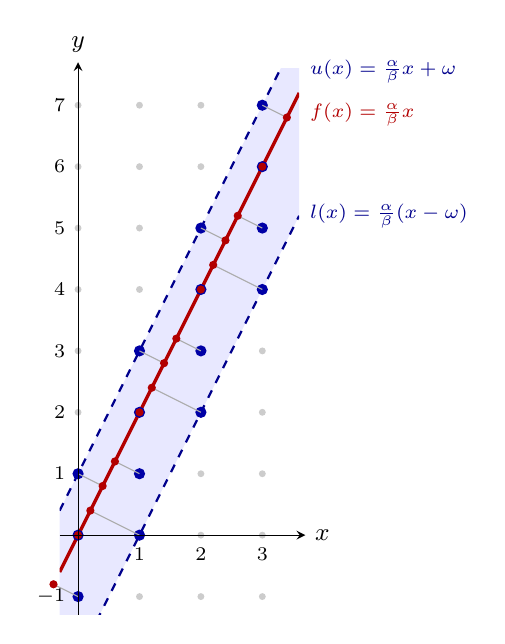
\begin{tikzpicture}[>=stealth, scale=0.78]

  % background lattice (faint gray)
  \foreach \x in {0,...,3} {
    \foreach \y in {-1,...,7} {
      \fill[gray!40] (\x,\y) circle (1.6pt);
    }
  }

  % strip shading (between l(x)=2x-2 and u(x)=2x+1)
  \begin{scope}
    \clip (-0.3,-1.3) rectangle (3.6,7.6);
    \fill[blue!9] (-0.3,-2.6) -- (-0.3,0.4) -- (3.6,8.2) -- (3.6,5.2) -- cycle;
  \end{scope}

  % strip boundaries and projection line (clipped)
  \begin{scope}
    \clip (-0.3,-1.3) rectangle (3.6,7.6);
    \draw[blue!55!black, thick, dashed] (-0.3, 0.4) -- (3.6, 8.2);   % u(x)
    \draw[blue!55!black, thick, dashed] (-0.3,-2.6) -- (3.6, 5.2);   % l(x)
    \draw[red!70!black,  very thick]    (-0.3,-0.6) -- (3.6, 7.2);   % f(x)
  \end{scope}

  % line labels (outside clip, near right edge)
  \node[font=\scriptsize, blue!55!black, anchor=west] at (3.62, 7.55)
    {$u(x)=\tfrac{\alpha}{\beta}x+\omega$};
  \node[font=\scriptsize, red!70!black,  anchor=west] at (3.62, 6.85)
    {$f(x)=\tfrac{\alpha}{\beta}x$};
  \node[font=\scriptsize, blue!55!black, anchor=west] at (3.62, 5.20)
    {$l(x)=\tfrac{\alpha}{\beta}(x-\omega)$};

  % accepted lattice points (large blue dots)
  \foreach \x/\y in {0/-1, 0/0, 0/1, 1/0, 1/1, 1/2, 1/3,
                     2/2, 2/3, 2/4, 2/5,
                     3/4, 3/5, 3/6, 3/7} {
    \fill[blue!65!black] (\x,\y) circle (2.6pt);
  }

  % orthogonal projection of every accepted point onto f(x)=2x
  % proj of (x,y) onto f(x)=2x is at ((x+2y)/5, 2(x+2y)/5)
  \foreach \x/\y in {0/-1, 0/0, 0/1, 1/0, 1/1, 1/2, 1/3,
                     2/2, 2/3, 2/4, 2/5,
                     3/4, 3/5, 3/6, 3/7} {
    \pgfmathsetmacro{\px}{(\x + 2*\y)/5}
    \pgfmathsetmacro{\py}{2*(\x + 2*\y)/5}
    \draw[gray!65, thin] (\x,\y) -- (\px,\py);
    \fill[red!70!black] (\px,\py) circle (1.9pt);
  }

  % axes
  \draw[->] (-0.3, 0) -- (3.7, 0) node[right, font=\small] {$x$};
  \draw[->] (0, -1.3) -- (0, 7.7) node[above, font=\small] {$y$};
  \foreach \x in {1,2,3}
    \node[below, font=\scriptsize] at (\x, -0.05) {$\x$};
  \foreach \y in {-1,1,2,3,4,5,6,7}
    \node[left, font=\scriptsize] at (-0.05, \y) {$\y$};

\end{tikzpicture}
\caption{Construction of the cut-and-project sequence for
  \(\alpha=2\), \(\beta=1\), \(\omega=1\).
  The strip (shaded) is bounded by the parallel lines
  \(u(x)=(\alpha/\beta)x+\omega\) and \(l(x)=(\alpha/\beta)(x-\omega)\).
  Accepted lattice points (filled blue dots) lie inside the strip; faint dots
  show rejected lattice points.  Each accepted point is projected orthogonally
  onto the line \(f(x)=(\alpha/\beta)x\) (red); the resulting projected points
  are drawn as red dots on \(f\), each connected to its preimage by a thin line.
  The ordered sequence of projected values
  \(\tilde{p}=\beta x+\alpha y\) defines the gap sequence studied in this paper.}
\label{fig:construction}
\end{figure}

\subsection{Multiplicity convention}\label{subsec:multiplicity}

There are two natural ways to enumerate the projected points along the
line, and we treat both in this paper.

\begin{description}
    \item[Multiset convention.]  Projected values are counted with
    multiplicity.  Thus, if two distinct accepted lattice points have the
    same projected coordinate, they contribute two consecutive entries to
    the sorted sequence and produce a zero gap.  Equivalently, we study the
    gap sequence of the projected lattice-point \emph{multiset}.

    \item[Set convention.]  Coincident projected values are identified, so
    each value occurs at most once in the sorted sequence.  Equivalently,
    we study the gap sequence of the underlying projected \emph{point
    set}.
\end{description}

\begin{figure}[ht]
\centering
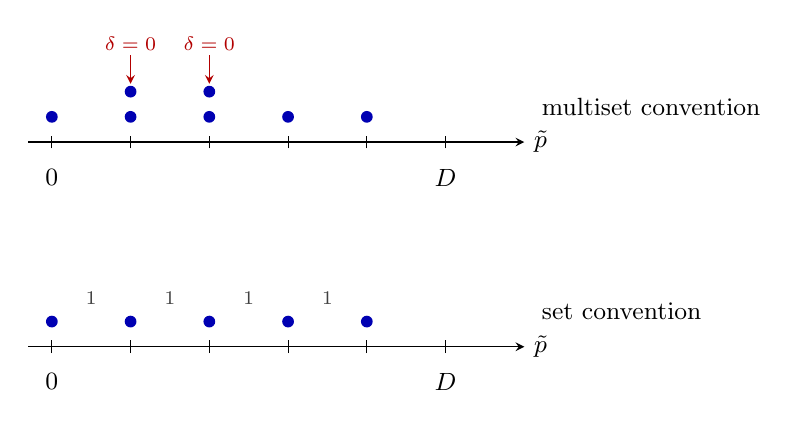
\begin{tikzpicture}[scale=1.0,
    pt/.style={circle,fill=blue!70!black,inner sep=1.5pt},
    axislabel/.style={font=\small},
    zerolabel/.style={font=\scriptsize,red!70!black},
    gaplabel/.style={font=\scriptsize,gray!50!black},
    >=stealth]

  \def\dy{0.32}

  % --- TOP PANEL: multiset ---
  \begin{scope}[yshift=2.6cm]
    \draw[->] (-0.3,0) -- (6.0,0) node[right,axislabel]{\(\tilde p\)};
    \foreach \x in {0,1,2,3,4,5} \draw (\x,-0.08) -- (\x,0.08);
    \node[below=4pt,axislabel] at (0,-0.08) {\(0\)};
    \node[below=4pt,axislabel] at (5,-0.08) {\(D\)};
    \foreach \x/\m in {0/1, 1/2, 2/2, 3/1, 4/1} {
      \foreach \k in {1,...,\m} {
        \pgfmathsetmacro{\y}{\dy*\k}
        \node[pt] at (\x,\y) {};
      }
    }
    \node[zerolabel] at (1,1.25) {\(\delta=0\)};
    \node[zerolabel] at (2,1.25) {\(\delta=0\)};
    \draw[red!70!black,thin,->,>=stealth]
         (1,1.10) -- (1,\dy*2+0.10);
    \draw[red!70!black,thin,->,>=stealth]
         (2,1.10) -- (2,\dy*2+0.10);
    \node[axislabel,anchor=west] at (6.1,0.45)
         {multiset convention};
  \end{scope}

  % --- BOTTOM PANEL: set ---
  \begin{scope}
    \draw[->] (-0.3,0) -- (6.0,0) node[right,axislabel]{\(\tilde p\)};
    \foreach \x in {0,1,2,3,4,5} \draw (\x,-0.08) -- (\x,0.08);
    \node[below=4pt,axislabel] at (0,-0.08) {\(0\)};
    \node[below=4pt,axislabel] at (5,-0.08) {\(D\)};
    \foreach \x in {0,1,2,3,4} \node[pt] at (\x,\dy) {};
    \foreach \x in {0,1,2,3} {
      \node[gaplabel] at (\x+0.5,\dy+0.30) {\(1\)};
    }
    \node[axislabel,anchor=west] at (6.1,0.45)
         {set convention};
  \end{scope}

\end{tikzpicture}
\caption{Multiset versus set convention on one length-\(D\) window of
the \(\tilde p\)-axis (here \(D=5\), with multiplicities
\((1,2,2,1,1)\), so \(N=7\); realizable for
\((\alpha,\beta)=(1,2)\) with \(\omega\in[2,5/2)\)).
Top: every accepted lattice point contributes a separate entry, so
coincident projected values produce \emph{zero gaps} (marked).
Bottom: identifying coincident values yields one entry per residue
class; here every class is hit, so all gaps equal~\(1\).}
\label{fig:multiset-vs-set}
\end{figure}

The two conventions can produce different period lengths, and we prove a
formula for each.  The main result for the multiset convention is
Theorem~\ref{thm:main} (Section~\ref{sec:mainresult}).  The companion
result for the set convention is Theorem~\ref{thm:setperiod}
(Section~\ref{sec:setvalued}).  In every case the set-valued period
divides the multiset period, with equality if and only if \(N \le D\); see
Corollary~\ref{cor:setlemultiset}.

Unless otherwise stated, the technical development in
Sections~\ref{sec:mainresult}--\ref{sec:degenerate} uses the multiset
convention.

\subsection{Gap sequence and period}\label{subsec:gapseq}

As shown below in Section~\ref{subsec:step2}, the projected values form a
finite union of arithmetic progressions with common difference
\(\alpha^2+\beta^2\), counted with finite multiplicities.  Hence the
resulting multiset is locally finite and unbounded in both directions.  It
therefore admits a nondecreasing enumeration indexed by \(\mathbb{Z}\),
unique up to translation of the index.

Sort the multiset of all \(\tilde{p}\)-values in nondecreasing order, with
multiplicities retained, to obtain
\((\tilde{p}^{(i)}_s)_{i \in \mathbb{Z}}\), and define the
\emph{gap sequence}
\begin{equation}\label{eq:delta}
    \delta^{(i)} \;:=\; \tilde{p}^{(i+1)}_s - \tilde{p}^{(i)}_s.
\end{equation}
Since orthogonal projection onto the line rescales the ordered
\(\tilde{p}\)-coordinate by a positive constant, the period length of
\((\delta^{(i)})\) equals the period length of the corresponding Euclidean
gap sequence between consecutive projected multiset entries, including
zero distances arising from coincident projected points.

\begin{definition}\label{def:period}
The sequence \((\delta^{(i)})_{i \in \mathbb{Z}}\) has \emph{period length}
\(\lambda \in \mathbb{N}\) if \(\lambda\) is the smallest positive integer
such that \(\delta^{(i+\lambda)} = \delta^{(i)}\) for all~\(i\).
\end{definition}

\subsection{\texorpdfstring{The trivial case \(\omega = 0\)}{The trivial case omega = 0}}\label{subsec:omega0}

When \(\omega = 0\), the only accepted lattice points lie on \(f\) itself:
\((x, y) = k(\beta, \alpha)\) for \(k \in \mathbb{Z}\).
Then
\[
    \tilde{p} = \beta \cdot k\beta + \alpha \cdot k\alpha
    = k(\alpha^2+\beta^2),
\]
so all differences equal \(\alpha^2+\beta^2\) and \(\lambda = 1\).
Note that the formula~\eqref{eq:formula} agrees: \(N = 0 + 0 + 1 = 1\)
and \(D = \alpha^2+\beta^2 \ge 2\), so \(D \nmid 1\) and \(\lambda = N = 1\).

% =====================================================================
\section{Main Result}\label{sec:mainresult}
% =====================================================================

\begin{theorem}[Period length formula]\label{thm:main}
Let \(\alpha, \beta \in \mathbb{N}\) with \(\gcd(\alpha, \beta) = 1\) and let
\(\omega \in \mathbb{R}_{\ge 0}\).  Define
\begin{equation}\label{eq:ND}
    N \;:=\; \lfloor\omega\alpha\rfloor + \lfloor\omega\beta\rfloor + 1,
    \qquad
    D \;:=\; \alpha^2 + \beta^2.
\end{equation}
Then the period length of the gap sequence~\eqref{eq:delta} is
\begin{equation}\label{eq:formula}
    \lambda_{\mathrm{multiset}} \;=\;
    \begin{cases}
        N   & \text{if } D \nmid N, \\
        N/D & \text{if } D \mid N.
    \end{cases}
\end{equation}
\end{theorem}

\begin{remark}[Interpretation of \(N\)]\label{rem:N}
The quantity \(N\) equals
\[
    \#\bigl([-\beta\omega,\,\alpha\omega]\cap\mathbb{Z}\bigr),
\]
the number of integers in the range of the invariant
\(r = \alpha x - \beta y\) (see Section~\ref{subsec:step1}).
Geometrically, \(N\) counts the number of tracks, namely the parallel arithmetic progressions of
projected values counted with multiplicity (see Figure~\ref{fig:tracks}).
\end{remark}

\begin{remark}[Interpretation of \(D\)]\label{rem:D}
The quantity \(D = \alpha^2+\beta^2\) is the common difference of each
arithmetic progression of \(\tilde{p}\)-values.
It also equals \(\lVert(\beta,\alpha)\rVert^2\), the squared length of the
direction vector of~\(f\).
\end{remark}

\begin{remark}[Computational verification]\label{rem:verification}
The multiset and set formulas have been verified jointly against the same
CSV datasets, since each row records both \(\lambda_{\mathrm{multiset}}\)
and \(\lambda_{\mathrm{set}}\):
\begin{itemize}
    \item 51{,}012 test cases with \(\alpha, \beta\) up to \({\sim}100{,}000\)
          and rational \(\omega\) up to \({\sim}10\), all satisfying
          \(D \nmid N\) (51{,}011 with \(N < D\), one with \(N \ge D\));
          see file \texttt{multiset\_\allowbreak and\_\allowbreak set\_\allowbreak new\_\allowbreak find\_\allowbreak patterns\_\allowbreak 51012\_\allowbreak lines.csv}
          in the repository's \texttt{tests/} folder.
    \item 477 cases at \((\alpha, \beta) = (1, 2)\) with rational \(\omega\)
          chosen so that \(D \mid N\) (with \(N\) up to \({\sim}4{,}300\)),
          verifying the \(\lambda = N/D\) branch; see file
          \texttt{multiset\_\allowbreak and\_\allowbreak set\_\allowbreak degenerate\_\allowbreak patterns\_\allowbreak 5000\_\allowbreak lines.csv}
          in the repository's \texttt{tests/} folder.
    \item 240 additional cases generated by an independent Python
          implementation, balanced 120 / 120 between \(N < D\) and
          \(N \ge D\) and spanning 25 distinct \((\alpha, \beta)\) pairs;
          see file \texttt{set\_\allowbreak theorem\_\allowbreak balanced\_\allowbreak test.csv}.
\end{itemize}
All 51{,}729 cases produce exact matches with zero failures for both the
multiset formula~\eqref{eq:formula} and the set formula~\eqref{eq:setformula}
(see Theorem~\ref{thm:setperiod} below).  These computations are used only
as consistency checks; the proofs below are independent of the empirical
verification.

Historically, the \(D \nmid N\) branch of the multiset
formula~\eqref{eq:formula} was first suggested by inspecting the datasets
at \(\omega = 1\), where
\(\lambda_{\mathrm{multiset}} = \alpha + \beta + 1\)
(see Corollary~\ref{cor:omega1}).

\end{remark}

% =====================================================================
\section{\texorpdfstring{Proof: The Generic Case \(D \nmid N\)}{Proof: The Generic Case D does not divide N}}\label{sec:proof}
% =====================================================================

\subsection{Step 1: Range of the invariant}\label{subsec:step1}

The strip condition~\eqref{eq:points}, multiplied by \(\beta > 0\), reads
\[
    \alpha(x - \omega) \;\le\; \beta y \;\le\; \alpha x + \beta\omega,
\]
equivalently
\begin{equation}\label{eq:r_range}
    -\beta\omega \;\le\;
    \underbrace{\alpha x - \beta y}_{=:\,r}
    \;\le\; \alpha\omega.
\end{equation}
Since \(r \in \mathbb{Z}\), it takes values in
\begin{equation}\label{eq:R}
    \mathcal{R} \;:=\;
    \bigl\{-\lfloor\beta\omega\rfloor,\;
    -\lfloor\beta\omega\rfloor + 1,\; \ldots,\;
    \lfloor\alpha\omega\rfloor\bigr\},
\end{equation}
using the identity \(\lceil{-x}\rceil = -\lfloor x \rfloor\).
Hence
\[
    |\mathcal{R}| =
    \lfloor\alpha\omega\rfloor + \lfloor\beta\omega\rfloor + 1 = N.
\]

The invariant \(r\) is constant along each track: if \((x, y)\) and
\((x + \beta, y + \alpha)\) are both accepted, they share the same~\(r\),
since
\[
    \alpha(x+\beta) - \beta(y+\alpha) = \alpha x - \beta y.
\]
The step \((\beta, \alpha)\) is the direction of~\(f\).

\begin{figure}[ht]
\centering
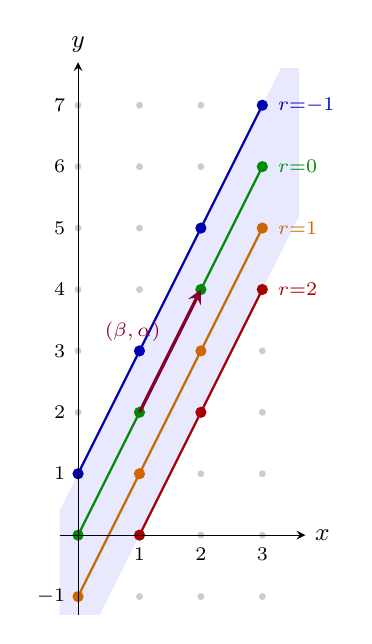
\begin{tikzpicture}[>=stealth, scale=0.78]

  % strip shading (same setup as Figure~\ref{fig:construction}: alpha=2, beta=1, omega=1)
  \begin{scope}
    \clip (-0.3,-1.3) rectangle (3.6,7.6);
    \fill[blue!9] (-0.3,-2.6) -- (-0.3,0.4) -- (3.6,8.2) -- (3.6,5.2) -- cycle;
  \end{scope}

  % faint background lattice
  \foreach \x in {0,...,3} {
    \foreach \y in {-1,...,7} {
      \fill[gray!40] (\x,\y) circle (1.6pt);
    }
  }

  % four track lines (one per value of r)
  \draw[blue!70!black,   thick] (0,1)   -- (3,7);   % r=-1: y=2x+1
  \draw[green!55!black,  thick] (0,0)   -- (3,6);   % r= 0: y=2x
  \draw[orange!80!black, thick] (0,-1) -- (3,5);   % r= 1: y=2x-1
  \draw[red!65!black,    thick] (1,0)   -- (3,4);   % r= 2: y=2x-2

  % accepted lattice points coloured by track
  \foreach \x/\y in {0/1, 1/3, 2/5, 3/7}
    \fill[blue!70!black]   (\x,\y) circle (2.6pt);
  \foreach \x/\y in {0/0, 1/2, 2/4, 3/6}
    \fill[green!55!black]  (\x,\y) circle (2.6pt);
  \foreach \x/\y in {0/-1, 1/1, 2/3, 3/5}
    \fill[orange!80!black] (\x,\y) circle (2.6pt);
  \foreach \x/\y in {1/0, 2/2, 3/4}
    \fill[red!65!black]    (\x,\y) circle (2.6pt);

  % r labels on the right
  \node[right, font=\scriptsize\bfseries, blue!70!black]
    at (3.10,7) {$r{=}{-1}$};
  \node[right, font=\scriptsize\bfseries, green!55!black]
    at (3.10,6) {$r{=}0$};
  \node[right, font=\scriptsize\bfseries, orange!80!black]
    at (3.10,5) {$r{=}1$};
  \node[right, font=\scriptsize\bfseries, red!65!black]
    at (3.10,4) {$r{=}2$};

  % direction (beta, alpha) arrow on track r=0
  \draw[->, very thick, purple!70!black] (1,2) -- (2,4);
  \node[above left, font=\scriptsize, purple!70!black] at (1.5,3)
    {$(\beta,\alpha)$};

  % axes
  \draw[->] (-0.3, 0) -- (3.7, 0) node[right, font=\small] {$x$};
  \draw[->] (0, -1.3) -- (0, 7.7) node[above, font=\small] {$y$};
  \foreach \x in {1,2,3}
    \node[below, font=\scriptsize] at (\x, -0.05) {$\x$};
  \foreach \y in {-1,1,2,3,4,5,6,7}
    \node[left, font=\scriptsize] at (-0.05, \y) {$\y$};

\end{tikzpicture}
\caption{The same setup as Figure~\ref{fig:construction}
  (\(\alpha = 2\), \(\beta = 1\), \(\omega = 1\)), now decomposed by the
  invariant \(r = \alpha x - \beta y\).  Each coloured line is a \emph{track}:
  the set of accepted lattice points sharing one value of \(r\).  The four
  admissible values \(r \in \{-1, 0, 1, 2\}\) give \(N = 4\) tracks, all
  parallel to the projection direction \((\beta, \alpha) = (1, 2)\) (purple
  arrow).  Step~2 of the proof shows that the projected
  \(\tilde{p}\)-values along a single track form an arithmetic progression
  with common difference \(D = \alpha^2 + \beta^2 = 5\).}
\label{fig:tracks}
\end{figure}

\subsection{\texorpdfstring{Step 2: Each value of \(r\) yields one arithmetic progression}{Step 2: Each value of r yields one arithmetic progression}}
\label{subsec:step2}

For a fixed \(r \in \mathcal{R}\), the system
\begin{equation}\label{eq:system}
    \beta x + \alpha y = \tilde{p}, \qquad
    \alpha x - \beta y = r
\end{equation}
has determinant \(-(\alpha^2+\beta^2) = -D \ne 0\), giving the unique solution
\begin{equation}\label{eq:solution}
    x = \frac{\beta\tilde{p} + \alpha r}{D}, \qquad
    y = \frac{\alpha\tilde{p} - \beta r}{D}.
\end{equation}
Integrality of \(x\) requires \(D \mid (\beta\tilde{p} + \alpha r)\), i.e.
\begin{equation}\label{eq:residue}
    \tilde{p} \;\equiv\; c_r \;:=\; -\alpha\beta^{-1}r \pmod{D},
\end{equation}
where \(\beta^{-1}\) is the modular inverse of \(\beta\) modulo \(D\).
The invertibility of \(\beta\) modulo \(D\) is proved in Corollary~\ref{cor:inverse}.
Throughout, we identify
\(c_r\) with its unique representative in \(\{0, 1, \ldots, D-1\}\),
so that expressions such as \(c_r + kD\) are well-defined integers.  Integrality of \(y\) is then
automatic: from~\eqref{eq:residue},
\[
    \alpha\tilde{p} - \beta r
    \;\equiv\;
    -\alpha^2\beta^{-1}r - \beta r
    \;=\;
    -(\alpha^2 + \beta^2)\beta^{-1}r
    \;\equiv\; 0 \pmod{D},
\]
so both coordinates in~\eqref{eq:solution} are integers.
The set of \(\tilde{p}\)-values for invariant~\(r\) is therefore the
arithmetic progression
\begin{equation}\label{eq:Pr}
    P_r \;=\; \{c_r + kD : k \in \mathbb{Z}\}.
\end{equation}
Conversely, if \(\tilde{p} \in P_r\), then the congruence
\eqref{eq:residue} makes both coordinates in~\eqref{eq:solution} integral,
and since \(r \in \mathcal{R}\), the resulting lattice point satisfies the
strip condition~\eqref{eq:r_range}.  Thus \(P_r\) is exactly the set of
\(\tilde{p}\)-values with invariant \(r\).  The complete multiset of
projected values is
\[
    S = \bigcup_{r \in \mathcal{R}} P_r,
\]
where the union is understood as a multiset union.

\subsection{Step 3: Coprimality lemmas}\label{subsec:step3}

\begin{lemma}\label{lem:gcd}
\(\gcd(\alpha, D) = \gcd(\beta, D) = 1\).
\end{lemma}

\begin{proof}
\(D = \alpha^2 + \beta^2 \equiv \beta^2 \pmod{\alpha}\), so any common
divisor of \(\alpha\) and \(D\) divides \(\beta^2\).  But
\(\gcd(\alpha,\beta)=1\) implies \(\gcd(\alpha,\beta^2)=1\).
The argument for \(\beta\) is symmetric.
\end{proof}

\begin{corollary}\label{cor:inverse}
The modular inverse \(\beta^{-1} \pmod{D}\) exists, and the map
\(r \mapsto c_r = -\alpha\beta^{-1}r \bmod D\) is a bijection on
\(\mathbb{Z}/D\mathbb{Z}\).
\end{corollary}

\begin{proof}
Lemma~\ref{lem:gcd} gives \(\gcd(\beta, D) = 1\), so \(\beta\) is a unit
modulo~\(D\).  By the same lemma \(\gcd(\alpha, D) = 1\), so the product
\(-\alpha\beta^{-1}\) is also a unit modulo~\(D\).  Multiplication by a
unit on \(\mathbb{Z}/D\mathbb{Z}\) is a bijection.
\end{proof}

\subsection{Step 4: Structure of residues}\label{subsec:step4}

The \(N\) residues \(\{c_r : r \in \mathcal{R}\}\) are the image of \(N\)
consecutive integers under multiplication by
\(m := -\alpha\beta^{-1} \bmod D\), with \(\gcd(m, D) = 1\).  Explicitly:
\begin{equation}\label{eq:residues}
    \{c_r\}_{r \in \mathcal{R}} \;=\;
    \{m \cdot r_0,\; m(r_0+1),\; \ldots,\; m(r_0+N-1)\} \bmod D,
\end{equation}
where \(r_0 = -\lfloor\beta\omega\rfloor\).

\begin{lemma}[Nonuniform residue distribution]\label{lem:nonuniform}
If \(D \nmid N\), the multiset of \(N\) residues
\(\{c_r \bmod D : r \in \mathcal{R}\}\) is not uniformly distributed over
\(\mathbb{Z}/D\mathbb{Z}\).  More precisely, writing \(N = qD + s\) with
\(0 < s < D\), exactly \(s\) residue classes are hit \(q+1\) times and
\(D - s\) residue classes are hit \(q\) times.
\end{lemma}

\begin{proof}
The map \(r \mapsto mr \bmod D\) is a bijection on
\(\mathbb{Z}/D\mathbb{Z}\) by Corollary~\ref{cor:inverse}.
As \(r\) runs through consecutive integers, the residues \(mr \bmod D\)
advance by the fixed unit \(m\); since \(\gcd(m, D) = 1\), every block of
\(D\) consecutive values of \(r\) hits each residue class exactly once.
After \(q\) complete cycles, all classes have been hit exactly \(q\) times.
The remaining \(s = N - qD\) values hit \(s\) additional classes exactly once
each.
Hence \(s\) classes have multiplicity \(q + 1\) and \(D - s\) classes have
multiplicity~\(q\).
\end{proof}

\begin{lemma}[Uniform residue distribution]\label{lem:uniform}
If \(D \mid N\), then every residue class \(c \in \mathbb{Z}/D\mathbb{Z}\) is
hit exactly \(N/D\) times by the multiset
\(\{c_r \bmod D : r \in \mathcal{R}\}\).
\end{lemma}

\begin{proof}
By Corollary~\ref{cor:inverse}, each block of \(D\) consecutive values of
\(r\) hits every residue class in \(\mathbb{Z}/D\mathbb{Z}\) exactly once.
Since \(D \mid N\), the \(N\) consecutive values of \(\mathcal{R}\) split
into \(N/D\) such blocks, so each class is hit exactly \(N/D\) times.
\end{proof}

\subsection{\texorpdfstring{Step 5: Period equals \(N\) when \(D \nmid N\)}{Step 5: Period equals N when D does not divide N}}
\label{subsec:step5}

The minimality argument relies on two self-contained facts; we state
them separately for reuse and clarity.

\begin{lemma}[Minimal period divides every period]
\label{lem:minperiod_divides_periods}
Let \((a_i)_{i\in\mathbb Z}\) be a bi-infinite sequence with minimal
positive period~\(\lambda\).  If \(M > 0\) is also a period, then
\(\lambda \mid M\).
\end{lemma}

\begin{proof}
Write \(M = q\lambda + r\) with \(0 \le r < \lambda\).  Both \(M\) and
\(\lambda\) are periods of the bi-infinite sequence; since the set of
periods is closed under both addition and subtraction (using negative
shifts where needed), the difference
\(M - q\lambda = r\) is itself a period of the sequence.  As
\(0 \le r < \lambda\) and \(\lambda\) is the \emph{minimal} positive
period, the only possibility is \(r = 0\); hence \(\lambda \mid M\).
\end{proof}

\begin{lemma}[Trivial stabilizer of a cyclic interval]
\label{lem:cyclic_interval_stabilizer}
Let \(0 < s < D\) and let
\[
    H = \{x_0,\, x_0+1,\, \ldots,\, x_0+s-1\} \pmod{D}
\]
be a cyclic interval of length \(s\) in \(\mathbb{Z}/D\mathbb{Z}\).
If \(\tau \in \mathbb{Z}/D\mathbb{Z}\) satisfies \(H + \tau = H\),
then \(\tau \equiv 0 \pmod{D}\).
\end{lemma}

\begin{proof}
The element \(x_0\) lies in \(H\) while \(x_0 - 1\) does not, so
\(x_0\) is the unique element of \(H\) whose predecessor is not in
\(H\).  If \(H + \tau = H\), then \(x_0 + \tau\) must have the same
property and therefore equals \(x_0\), giving
\(\tau \equiv 0 \pmod{D}\).
\end{proof}

\begin{proposition}\label{prop:generic_period}
If \(D \nmid N\), then the multiset gap sequence has minimal
period \(\lambda = N\).
\end{proposition}

\begin{proof}
Within each interval \([kD,\,(k+1)D)\) on the \(\tilde{p}\)-axis, exactly
\(N\) points from the multiset \(S\) occur, counted with multiplicity.
Their positions within the interval are determined by the residues
\(c_r \bmod D\), again counted with multiplicity.

Let
\[
    0 \le v_0 \le v_1 \le \cdots \le v_{N-1} < D
\]
be the nondecreasing list of these residues in one interval of length \(D\),
with repetitions according to their multiplicities.  Then the sorted
projected multiset is obtained by repeating this same residue block in every
translate by \(D\).  More explicitly, after a possible translation of the
indexing, every \(i \in \mathbb Z\) can be written uniquely as
\[
    i = kN + j,
    \qquad
    k\in\mathbb Z,\quad 0\le j<N,
\]
and
\[
    \tilde{p}_s^{(i)} = kD + v_j.
\]
Consequently,
\[
    \tilde{p}_s^{(i+N)}
    =
    \tilde{p}_s^{(i)} + D
\]
for all \(i\in\mathbb Z\).  Therefore
\[
    \delta^{(i+N)}
    =
    \tilde{p}_s^{(i+N+1)}-\tilde{p}_s^{(i+N)}
    =
    \tilde{p}_s^{(i+1)}-\tilde{p}_s^{(i)}
    =
    \delta^{(i)}
\]
for all \(i\).  Thus \(N\) is a period of the gap sequence, and hence
by Lemma~\ref{lem:minperiod_divides_periods} the minimal period
\(\lambda\) divides \(N\).

\medskip
\noindent\textbf{Minimality.}
We now prove that no proper divisor of \(N\) is a period, using a
multiplicity-function argument on \(\mathbb{Z}/D\mathbb{Z}\).  Since the
multiset of residues comes from \(N\) consecutive integers under
multiplication by the unit \(m\), it is convenient to relabel coordinates
so that the heavy classes form a contiguous interval; the contradiction
will then follow from the fact that a proper cyclic interval has only the
trivial translational symmetry
(Lemma~\ref{lem:cyclic_interval_stabilizer}).

Define the multiplicity function
\[
    \mu \colon \mathbb{Z}/D\mathbb{Z} \to \mathbb{N}_0
\]
by
\[
    \mu(c) \;:=\; \bigl|\{r \in \mathcal{R} : c_r \equiv c \pmod{D}\}\bigr|.
\]
By Lemma~\ref{lem:nonuniform}, with \(N = qD + s\) and \(0 < s < D\),
the function \(\mu\) takes exactly two values: \(q+1\) on a set of \(s\)
residue classes and \(q\) on the remaining \(D - s\) classes.

It is convenient to pass to the \(m\)-stepping parametrization
\[
    f(x) := \mu(mx), \qquad x \in \mathbb{Z}/D\mathbb{Z},
\]
where \(m=-\alpha\beta^{-1}\pmod D\).
Since \(m\) is invertible modulo \(D\), this is only a relabeling of the
same data.  In this parametrization, the heavy set
\[
    H := \{x \in \mathbb{Z}/D\mathbb{Z} : f(x)=q+1\}
\]
is a contiguous cyclic interval of length \(s\):
\[
    H = \{x_0, x_0+1, \ldots, x_0+s-1\}\pmod D
\]
for some \(x_0\), because after \(q\) complete cycles the remaining
\(s\) elements contribute one additional hit on \(s\) consecutive
classes in the \(m\)-stepping order.

\begin{figure}[ht]
\centering
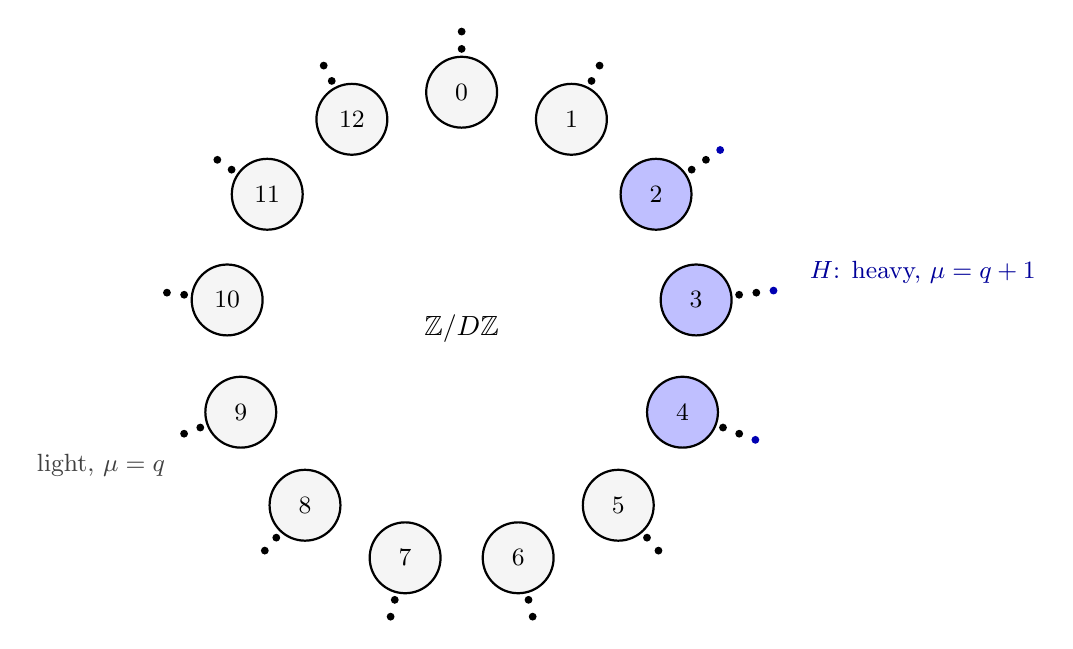
\begin{tikzpicture}[scale=1.0,
    heavy/.style={circle,draw,thick,fill=blue!25,minimum size=9mm,inner sep=0pt,font=\small},
    light/.style={circle,draw,thick,fill=gray!8,minimum size=9mm,inner sep=0pt,font=\small},
    dot/.style={circle,fill=black,inner sep=1pt},
    >=stealth]

  \def\R{3.0}
  \def\rtwr{0.55}

  \foreach \i/\style in {%
      0/light, 1/light, 2/heavy, 3/heavy, 4/heavy,
      5/light, 6/light, 7/light, 8/light, 9/light,
      10/light, 11/light, 12/light} {
    \pgfmathsetmacro{\ang}{90 - 360*\i/13}
    \node[\style] (n\i) at (\ang:\R) {\i};
  }

  \foreach \i in {0,1,...,12} {
    \pgfmathsetmacro{\ang}{90 - 360*\i/13}
    \pgfmathsetmacro{\rA}{\R+\rtwr}
    \pgfmathsetmacro{\rB}{\R+\rtwr+0.22}
    \node[dot] at (\ang:\rA) {};
    \node[dot] at (\ang:\rB) {};
  }

  \foreach \i in {2,3,4} {
    \pgfmathsetmacro{\ang}{90 - 360*\i/13}
    \pgfmathsetmacro{\rC}{\R+\rtwr+0.44}
    \node[dot,fill=blue!70!black] at (\ang:\rC) {};
  }

  \node[blue!60!black,font=\small] at (90-360*3/13:\R+2.9)
       {\(H\): heavy, \(\mu=q+1\)};
  \node[gray!50!black,font=\small] at (90-360*9/13:\R+1.9)
       {light, \(\mu=q\)};

  \node at (0,0) {\(\mathbb{Z}/D\mathbb{Z}\)};

\end{tikzpicture}
\caption{Heavy set \(H\subset\mathbb{Z}/D\mathbb{Z}\) in the
\(m\)-stepping parametrization
(here \(D=13,\ q=2,\ s=3,\ N=qD+s=29\); realizable for
\((\alpha,\beta,\omega)=(2,3,17/3)\)).
Next to each residue class, the multiplicity \(\mu\) is shown as a
small outward stack of dots: \(q=2\) for light classes, \(q+1=3\) for heavy
classes.  The heavy set \(H=\{2,3,4\}\) is a contiguous cyclic
interval of length \(s\).}
\label{fig:heavy-set}
\end{figure}

Now suppose, for contradiction, that the minimal period \(\lambda_0\) satisfies
\(\lambda_0 < N\).  Since \(N\) is a period, by
Lemma~\ref{lem:minperiod_divides_periods} the minimal period divides
\(N\).  Thus we may write
\[
    N = k\lambda_0
\]
with \(k>1\).

Let
\[
    \sigma := \delta^{(0)} + \delta^{(1)} + \cdots + \delta^{(\lambda_0-1)}.
\]
By \(\lambda_0\)-periodicity, every block of \(\lambda_0\) consecutive
gaps has the same sum \(\sigma\); that is, for every
\(i \in \mathbb{Z}\),
\[
    \delta^{(i)} + \delta^{(i+1)} + \cdots + \delta^{(i+\lambda_0-1)}
    = \sigma.
\]
Hence
\[
    \tilde{p}_s^{(i+\lambda_0)} = \tilde{p}_s^{(i)} + \sigma
\]
for all \(i\).  Since \(i \mapsto i+\lambda_0\) is a bijection of
\(\mathbb{Z}\), this translation maps the enumerated multiset
bijectively onto itself and preserves multiplicities; equivalently,
the entire multiset \(S\) is invariant under translation
by \(\sigma\).

On the other hand, \(N\) consecutive gaps always sum to \(D\), because
\[
    \tilde{p}_s^{(i+N)}-\tilde{p}_s^{(i)} = D.
\]
Since \(N=k\lambda_0\), this gives
\[
    k\sigma = D.
\]
Thus \(\sigma = D/k\) is a positive integer (positive because \(D>0\)
and \(k\ge 1\)) and \(k\mid D\).  In particular \(0 < \sigma < D\),
since \(k>1\).

Since translation by an integer \(\sigma\) sends an integer \(\tilde p\)
with residue class \(c \bmod D\) to the integer \(\tilde p + \sigma\)
with residue class \((c + \sigma) \bmod D\), the translation invariance
of \(S\) by \(\sigma\) implies invariance of the residue multiplicity
function:
\[
    \mu(c+\sigma)=\mu(c) \qquad \text{for all } c\in \mathbb{Z}/D\mathbb{Z}.
\]
Equivalently, the relabeled function \(f\) satisfies
\[
    f(x+\tau)=f(x), \qquad \tau := m^{-1}\sigma \pmod D.
\]
Since \(m\) is invertible modulo~\(D\) and \(0<\sigma<D\), we have
\(\tau\not\equiv 0\pmod D\).
Therefore its heavy set \(H\) must satisfy \(H+\tau = H\).

But \(H\) is a cyclic interval of length \(s\) with \(0 < s < D\), so
by Lemma~\ref{lem:cyclic_interval_stabilizer} the equality
\(H + \tau = H\) forces \(\tau \equiv 0 \pmod{D}\).

This contradiction shows that no proper divisor \(\lambda_0 < N\) can be a
period.  Since \(N\) is a period, it follows that the minimal period is
\[
    \lambda = N.
\]
\end{proof}

% =====================================================================
\section{\texorpdfstring{The Degenerate Case \(D \mid N\)}{The Degenerate Case D divides N}}\label{sec:degenerate}
% =====================================================================

\begin{theorem}\label{thm:degenerate}
If \(D \mid N\), then \(\lambda = N/D\).
\end{theorem}

\begin{proof}
By Lemma~\ref{lem:uniform}, every residue class
\(c \in \mathbb{Z}/D\mathbb{Z}\) is hit exactly \(N/D\) times.  Consequently,
each residue class contributes \(N/D\) projected multiset entries per
interval of length~\(D\) on the \(\tilde{p}\)-axis, and every integer
\(\tilde{p}\) is achieved with multiplicity~\(N/D\).

The sorted sequence of \(\tilde{p}\)-values, counted with multiplicity, thus
consists of each integer repeated \(N/D\) times:
\[
    \ldots,\;
    \underbrace{t,\, t,\, \ldots,\, t}_{N/D},\;
    \underbrace{t+1,\, t+1,\, \ldots,\, t+1}_{N/D},\;
    \ldots
\]
The gap sequence is
\[
    \underbrace{0,\, 0,\, \ldots,\, 0}_{N/D - 1},\; 1,\;
    \underbrace{0,\, 0,\, \ldots,\, 0}_{N/D - 1},\; 1,\;
    \ldots
\]
which has period \(N/D\).  This period is also minimal: if
\(N/D = 1\), the constant sequence has minimal period~\(1\); if
\(N/D > 1\), the value~\(1\) occurs exactly once in each block of
length \(N/D\) while all other entries in the block are~\(0\), so no
smaller positive period can preserve the positions of the entries
equal to~\(1\).  Hence the minimal period is~\(N/D\).
\end{proof}

\begin{proof}[Proof of Theorem~\ref{thm:main}]
If \(D \nmid N\), Proposition~\ref{prop:generic_period} gives
\(\lambda_{\mathrm{multiset}} = N\). If \(D \mid N\),
Theorem~\ref{thm:degenerate} gives \(\lambda_{\mathrm{multiset}} = N/D\).
The two cases together yield the formula~\eqref{eq:formula}.
\end{proof}

\begin{example}\label{ex:degenerate}
For \(\alpha = 2\), \(\beta = 1\), \(\omega = 3\):
\[
    N = \lfloor 6 \rfloor + \lfloor 3 \rfloor + 1 = 10,
    \qquad
    D = 5.
\]
Since \(5 \mid 10\), the formula gives \(\lambda = 10/5 = 2\).
Direct computation confirms the gap sequence
\((0, 1, 0, 1, \ldots)\) with period~\(2\).
\end{example}

\begin{example}\label{ex:degenerate2}
For \(\alpha = 3\), \(\beta = 2\), \(\omega = 5\):
\[
    N = \lfloor 15 \rfloor + \lfloor 10 \rfloor + 1 = 26,
    \qquad
    D = 13.
\]
Since \(13 \mid 26\), the formula gives \(\lambda = 26/13 = 2\).
\end{example}

\begin{remark}\label{rem:boundary}
The boundary case \(N = D\), i.e. \(N/D = 1\), gives
\(\lambda_{\mathrm{multiset}} = 1\): every integer is a projected value in
the \(\tilde{p}\)-coordinate with multiplicity~\(1\), and all gaps
equal~\(1\).  At this boundary the multiset and set conventions agree
(Theorem~\ref{thm:setperiod}, case \(N \ge D\); see also
Corollary~\ref{cor:setlemultiset}).
\end{remark}

% =====================================================================
\section{The Set-Valued Period}\label{sec:setvalued}
% =====================================================================

We now treat the set convention introduced in
Section~\ref{subsec:multiplicity}: coincident projected points are
identified, so each \(\tilde{p}\)-value occurs at most once in the sorted
sequence.

\subsection{Definition of the set-valued gap sequence}\label{subsec:setdef}

Sort the set of all values \(\tilde{p}\in\mathbb{Z}\) that occur as
projected values in increasing order, with each value listed once.
By Section~\ref{subsec:step2} this set is locally finite and unbounded in
both directions, so it admits a strictly increasing enumeration indexed by
\(\mathbb{Z}\), unique up to translation of the index.  Write this
enumeration \((\tilde{p}^{(i)}_{\mathrm{set}})_{i \in \mathbb{Z}}\) and
define the \emph{set-valued gap sequence}
\begin{equation}\label{eq:delta_set}
    \delta^{(i)}_{\mathrm{set}}
    \;:=\; \tilde{p}^{(i+1)}_{\mathrm{set}} - \tilde{p}^{(i)}_{\mathrm{set}}.
\end{equation}
Its minimal period \(\lambda_{\mathrm{set}}\) is defined exactly as in
Definition~\ref{def:period}.

\subsection{Statement and proof}

\begin{theorem}[Set-valued period]\label{thm:setperiod}
Let \(\alpha, \beta \in \mathbb{N}\) with \(\gcd(\alpha,\beta) = 1\) and
\(\omega \in \mathbb{R}_{\ge 0}\).  With \(N\) and \(D\) as
in~\eqref{eq:ND}, the set-valued gap sequence~\eqref{eq:delta_set}
has minimal period
\begin{equation}\label{eq:setformula}
    \lambda_{\mathrm{set}} \;=\;
    \begin{cases}
        N & \text{if } N < D, \\
        1 & \text{if } N \ge D.
    \end{cases}
\end{equation}
\end{theorem}

\begin{proof}
Write \(N = qD + s\) with \(0 \le s < D\) as in
Section~\ref{subsec:step5}, and
let \(\mu \colon \mathbb{Z}/D\mathbb{Z} \to \mathbb{N}_0\) be the
multiplicity function defined there.

\smallskip
\noindent\emph{Case \(N < D\).}  Then \(q = 0\), so by
Lemma~\ref{lem:nonuniform} the function \(\mu\) takes values in
\(\{0, 1\}\): exactly \(N\) residue classes are hit once, and the
remaining \(D - N\) are hit zero times.  Hence in the bi-infinite multiset
no integer occurs with multiplicity greater than one, and the underlying
set coincides with the multiset (as \(\mathbb{Z}\)-indexed sequences,
after a possible translation of the index).  In particular
\(\lambda_{\mathrm{set}} = \lambda_{\mathrm{multiset}}\).  Since
\(0 < N < D\) implies \(D \nmid N\), Theorem~\ref{thm:main} gives
\(\lambda_{\mathrm{multiset}} = N\).  Thus
\(\lambda_{\mathrm{set}} = N\).

\smallskip
\noindent\emph{Case \(N \ge D\).}  Then \(q \ge 1\), so by
Lemma~\ref{lem:nonuniform} (if \(D \nmid N\)) and
Lemma~\ref{lem:uniform} (if \(D \mid N\)), the function \(\mu\) takes
only positive values.  Hence every residue class is hit at least once,
and by~\eqref{eq:Pr} every integer is a projected value in the
\(\tilde{p}\)-coordinate.  The underlying set is therefore \(\mathbb{Z}\)
in the \(\tilde{p}\)-coordinate, its gap sequence in this coordinate is
constantly \(1\), and \(\lambda_{\mathrm{set}} = 1\).
\qedhere
\end{proof}

\subsection{Comparison with the multiset period}

\begin{corollary}\label{cor:setlemultiset}
For all \(\alpha, \beta, \omega\) as above,
\[
    \lambda_{\mathrm{set}} \;\mid\; \lambda_{\mathrm{multiset}},
\]
and in particular
\[
    \lambda_{\mathrm{set}} \;\le\; \lambda_{\mathrm{multiset}},
\]
with equality if and only if \(N \le D\).
\end{corollary}

\begin{proof}
Compare~\eqref{eq:formula} and~\eqref{eq:setformula} on the three
sub-regimes:
\begin{itemize}
    \item \(N < D\) (in particular \(D \nmid N\)):
          \(\lambda_{\mathrm{multiset}} = N = \lambda_{\mathrm{set}}\).
    \item \(N = D\) (so \(D \mid N\)):
          \(\lambda_{\mathrm{multiset}} = N/D = 1 = \lambda_{\mathrm{set}}\).
    \item \(N > D\): if \(D \mid N\) then
          \(\lambda_{\mathrm{multiset}} = N/D \ge 2 > 1
          = \lambda_{\mathrm{set}}\); if \(D \nmid N\) then
          \(\lambda_{\mathrm{multiset}} = N > 1 = \lambda_{\mathrm{set}}\).
\end{itemize}
In every case \(\lambda_{\mathrm{set}} \in \{1, \lambda_{\mathrm{multiset}}\}\),
which gives both \(\lambda_{\mathrm{set}} \mid \lambda_{\mathrm{multiset}}\)
(since \(1\) divides every positive integer) and the inequality, with
equality precisely when \(N \le D\).
\end{proof}

\subsection{Examples}

\begin{example}[\(N < D\), set and multiset agree]\label{ex:set_lt}
For \(\alpha = 2\), \(\beta = 3\), \(\omega = 2\): \(N = 4 + 6 + 1 = 11\)
and \(D = 13\), so \(N < D\).  Then
\(\lambda_{\mathrm{multiset}} = \lambda_{\mathrm{set}} = 11\).
\end{example}

\begin{example}[\(N = D\), boundary]\label{ex:set_eq}
For \(\alpha = 2\), \(\beta = 1\), \(\omega = 3/2\): \(N = 5 = D\), so
\(\lambda_{\mathrm{multiset}} = N/D = 1 = \lambda_{\mathrm{set}}\)
(cf.\ Remark~\ref{rem:boundary}).
\end{example}

\begin{example}[\(N > D\), \(D \nmid N\), set and multiset disagree]
\label{ex:set_gt}
Take \(\alpha = 3\), \(\beta = 4\), \(\omega = 4\).  Then
\[
    N = \lfloor 12 \rfloor + \lfloor 16 \rfloor + 1 = 29,
    \qquad
    D = 9 + 16 = 25,
    \qquad
    N = 1 \cdot D + 4,
\]
so the residue distribution
(Lemma~\ref{lem:nonuniform}) hits exactly \(4\) classes with
multiplicity \(2\) and the remaining \(21\) classes with
multiplicity \(1\).

\medskip
\noindent\emph{Multiset side.}  Within each length-\(D\) window of the
\(\tilde{p}\)-axis, the \(N = 29\) projected entries (counted with
multiplicity) include four duplicated values: each of the four
heavy residue classes contributes a coincident pair, hence a zero
gap.  The block of \(N\) gaps therefore contains four \(0\)'s and
\(N - 4 = 25\) positive values, summing to \(D\).
Theorem~\ref{thm:main} gives
\(\lambda_{\mathrm{multiset}} = N = 29\), and the heavy classes form
a cyclic interval of length \(s = 4\) whose only translational
symmetry is the identity
(Lemma~\ref{lem:cyclic_interval_stabilizer}).

\medskip
\noindent\emph{Set side.}  Since every residue class is hit at least
once, the underlying point set is all of \(\mathbb{Z}\) in the
\(\tilde{p}\)-coordinate.  Discarding multiplicities collapses the four
zero gaps and leaves the constant gap sequence \(1, 1, 1, \ldots\);
Theorem~\ref{thm:setperiod} gives
\(\lambda_{\mathrm{set}} = 1\).  Direct computation confirms both
values.
\end{example}

\subsection{Computational verification}\label{subsec:set_empirical}

The dichotomy \(N < D\) versus \(N \ge D\) is verified by the same datasets
listed in Remark~\ref{rem:verification}, since each row of those CSVs
records \(\lambda_{\mathrm{set}}\) alongside \(\lambda_{\mathrm{multiset}}\).
All 51{,}729 cases match formula~\eqref{eq:setformula} with zero failures.

% =====================================================================
\section{Corollaries}\label{sec:corollaries}
% =====================================================================

Throughout this section, \(\lambda\) denotes the multiset period
\(\lambda_{\mathrm{multiset}}\) of Theorem~\ref{thm:main}; the
set-valued analogues follow from Theorem~\ref{thm:setperiod} via
Corollary~\ref{cor:setlemultiset}.  Define
\(\Lambda_{\alpha,\beta} := \alpha + \beta + 1\).

\begin{corollary}[Finiteness]\label{cor:finite}
For all \(\alpha, \beta \in \mathbb{N}\) with \(\gcd(\alpha,\beta)=1\) and
all \(\omega \in \mathbb{R}_{\ge 0}\), the period length~\(\lambda\) is
finite.
\end{corollary}

\begin{proof}
\(N\) is a finite positive integer, and \(\lambda \le N\).
\end{proof}

\begin{corollary}[Period at \(\omega = 1\)]\label{cor:omega1}
For \(\omega = 1\), \(\lambda = \Lambda_{\alpha,\beta}\).

\end{corollary}

\begin{proof}
\(N = \alpha + \beta + 1\) and \(D = \alpha^2+\beta^2\).
For \((\alpha,\beta) \ne (1,1)\), we have
\[
    \alpha+\beta+1 < \alpha^2+\beta^2,
\]
so \(D \nmid N\) and \(\lambda = N = \alpha+\beta+1\).
For \((\alpha,\beta) = (1,1)\), \(N = 3\), \(D = 2\), and again
\(D \nmid N\), so \(\lambda = 3 = \Lambda_{1,1}\).
\end{proof}

\begin{corollary}[\(0 < \omega < 1\)]\label{cor:small_omega}
If \(0 < \omega < 1\), then
\[
    \lambda < \Lambda_{\alpha,\beta}.
\]
\end{corollary}

\begin{proof}
\(\lfloor\omega\alpha\rfloor \le \alpha - 1\) and
\(\lfloor\omega\beta\rfloor \le \beta - 1\), so
\[
    N \le \alpha + \beta - 1 < \Lambda_{\alpha,\beta}.
\]
Since \(\alpha + \beta - 1 < \alpha^2 + \beta^2 = D\) for all
\(\alpha, \beta \ge 1\), we have \(N < D\), hence \(D \nmid N\) and
\[
    \lambda = N < \Lambda_{\alpha,\beta}.
\]
\end{proof}

\begin{corollary}[\(1 < \omega < 2\)]\label{cor:medium_omega}
If \(1 < \omega < 2\) and \(D \nmid N\), then
\[
    \lambda \ge \Lambda_{\alpha,\beta}.
\]
\end{corollary}

\begin{proof}
\(\lfloor\omega\alpha\rfloor \ge \alpha\) and
\(\lfloor\omega\beta\rfloor \ge \beta\), so
\[
    N \ge \alpha + \beta + 1 = \Lambda_{\alpha,\beta}.
\]
Since \(D \nmid N\), we have \(\lambda = N \ge \Lambda_{\alpha,\beta}\).
\end{proof}

\begin{remark}
The condition \(D \nmid N\) in Corollary~\ref{cor:medium_omega} cannot be
dropped.  For \(\alpha = 2\), \(\beta = 1\), \(\omega = 3/2\), one has
\[
    N = \lfloor 3 \rfloor + \lfloor 3/2 \rfloor + 1 = 5 = D.
\]
Since \(D \mid N\), we get \(\lambda = N/D = 1\), which is less than
\(\Lambda_{2,1} = 4\).
\end{remark}

\begin{corollary}[\(\omega > 2\)]\label{cor:large_omega}
If \(\omega > 2\) and \(D \nmid N\), then
\[
    \lambda > \Lambda_{\alpha,\beta}.
\]
\end{corollary}

\begin{proof}
\(\lfloor\omega\alpha\rfloor \ge 2\alpha\) and
\(\lfloor\omega\beta\rfloor \ge 2\beta\), so
\[
    N \ge 2\alpha + 2\beta + 1 > \Lambda_{\alpha,\beta}.
\]
Since \(D \nmid N\), \(\lambda = N > \Lambda_{\alpha,\beta}\).
\end{proof}

\begin{remark}
In both corollaries above, the degenerate case \(D \mid N\) can produce
small periods: \(\lambda = N/D\) may be much less than
\(\Lambda_{\alpha,\beta}\).  This occurs when the window parameter is tuned so
that the number of tracks is an exact multiple of \(D = \alpha^2+\beta^2\).
\end{remark}

% =====================================================================
\section{The Irrational Case}\label{sec:irrational}
% =====================================================================

The body of this paper concerns positive rational slopes \(\alpha/\beta\).
For completeness we record the complementary regime of irrational slopes,
where the projected gap sequence fails to be periodic.  This statement is
not a corollary of Theorem~\ref{thm:main}; we include it to make the
periodic--aperiodic boundary explicit.

In this section we momentarily replace the rational invariants \(r\),
\(\tilde p\), \(\mathcal{R}\) by the standard physical/internal coordinates
\(\tilde p, s\) of cut-and-project theory; the rational analogues are
recovered by setting \(a = \alpha/\beta\).%
\footnote{Note that the symbol \(\tilde p\) is reused with a different
normalization: in \S\ref{subsec:projection} we set
\(\tilde p = \beta x + \alpha y\), whereas here \(\tilde p = x + a y\).
With \(a=\alpha/\beta\), the irrational form is the rational form divided
by the positive constant~\(\beta\), so the two definitions induce the same
ordering of projected points.}

Throughout this section we use the following notation.  For irrational
\(a\) and \(\omega > 0\), define the physical and internal coordinates
\[
    \tilde p(x, y) \;:=\; x + a y,
    \qquad
    s(x, y) \;:=\; y - a x,
\]
the internal window
\[
    W \;:=\; [-a\omega,\, \omega],
\]
and the set of accepted lattice points
\[
    A \;:=\; \bigl\{(x, y) \in \mathbb{Z}^2 : s(x, y) \in W\bigr\}.
\]
The strip condition \(a(x-\omega)\le y \le ax+\omega\) is equivalent to
\(s(x, y) \in W\), so \(A\) is precisely the set of points accepted by
the irrational strip projection.

The strip has bounded internal-coordinate width given by \(W\), and
\(\tilde p\) and \(s\) are linearly independent forms on \(\mathbb{R}^2\).
Consequently, the intersection of the strip with the preimage of any
bounded \(\tilde p\)-interval is a bounded parallelogram in
\(\mathbb{R}^2\) and hence contains only finitely many lattice points;
the projected set \(\tilde p(A)\) is therefore locally finite.

Unboundedness in both directions follows from a lattice-translate
construction whose quantifier structure is the natural one for a
Diophantine-style argument: given any target \(M \in \mathbb{R}\), the
base lattice vector \((p_0, q_0)\) and the scaling integer \(K\) are
both chosen depending on~\(M\).

Fix the target \(M \in \mathbb{R}\), set
\(c_0 := 1 + a^2 - |a|\) (strictly positive since
\(c_0 = (|a| - \tfrac12)^2 + \tfrac34 \ge \tfrac34\)),
and choose%
\footnote{This matches the auxiliary parameter built with
\(\min 1(\cdots)\) in \texttt{exists\_scaled\_witness}
(\texttt{Irrational.lean}).}
\[
    0 \;<\; \varepsilon \;\le\;
    \min\!\bigl(1,\;
      c_0 \min(a\omega, \omega) / (|M| + 2 c_0 + 1)\bigr).
\]

By density of \(s(\mathbb{Z}^2) = \{n - a m : m, n \in \mathbb{Z}\}\) in
\(\mathbb{R}\) (see Step~3 of the proof of
Proposition~\ref{prop:irrational} below), there exists
\((p_0, q_0) \in \mathbb{Z}^2\) with
\(0 < |s(p_0, q_0)| < \varepsilon\).  Since \(\varepsilon \le 1\), the
relation \(s(p_0, q_0) = q_0 - a p_0\) with \(|s(p_0, q_0)| < 1\) forces
\(p_0 \ne 0\) (else \(|q_0| < 1\) would give \(q_0 = 0\), contradicting
\(|s(p_0, q_0)| > 0\)).  Hence \(|p_0| \ge 1\), and the identity
\[
    \tilde p(p_0, q_0) \;=\; (1 + a^2)\, p_0 + a\, s(p_0, q_0)
\]
yields the uniform lower bound \(|\tilde p(p_0, q_0)| \ge c_0\).
Replacing \((p_0, q_0)\) by \((-p_0, -q_0)\) if necessary, we may assume
\(\tilde p(p_0, q_0) \ge c_0\).  Setting
\[
    K \;:=\; \max\!\bigl(1,\;\lceil M / \tilde p(p_0, q_0) \rceil + 1\bigr)
    \;\in\;\mathbb{Z}_{>0},
\]
the lower bound \(\tilde p(p_0, q_0) \ge c_0 > 0\) gives the explicit
estimate \(K \le |M|/c_0 + 2\) (the \(\max\) prevents \(K\) from going
negative when \(M\) is large negative, while the inequality
\(K \cdot \tilde p(p_0, q_0) > M\) still holds in both branches: the
branch \(K = 1\) is used precisely when \(\lceil M/\tilde p(p_0,q_0)\rceil
\le 0\), i.e.\ when \(M \le 0\), so \(K \tilde p(p_0,q_0) = \tilde
p(p_0,q_0) \ge c_0 > 0 \ge M\)).  The bound on \(\varepsilon\) then
ensures
\(|s(K p_0, K q_0)| = K \cdot |s(p_0, q_0)| < K \varepsilon
  \le \min(a\omega, \omega)\),
hence \(s(K p_0, K q_0) \in W\) and \((K p_0, K q_0) \in A\);
meanwhile
\(\tilde p(K p_0, K q_0) = K \cdot \tilde p(p_0, q_0) > M\).  The
negative direction is symmetric: the bound on \(|s(K p_0, K q_0)|\) is
symmetric in sign, so the negated point \((-K p_0, -K q_0)\) also
satisfies \(|s(-K p_0, -K q_0)| < \min(a\omega, \omega)\) and therefore
lies in \(A\) (even though \(W\) itself is asymmetric when \(a\ne 1\)).
Applying the construction to \(-M\) in place of \(M\) and negating the
resulting lattice point thus produces a member of \(A\) with
\(\tilde p\)-value below \(M\).  The gap sequence is therefore
well defined via the increasing \(\mathbb{Z}\)-indexed enumeration of
\(\tilde p(A)\).  (The same construction, with explicit constants, is
used in the Lean formalization to discharge \texttt{NoMaxOrder} and
\texttt{NoMinOrder} on \(\tilde p(A)\); see
\texttt{exists\_scaled\_witness} in \texttt{Irrational.lean}.)

\begin{proposition}[Aperiodicity for irrational slope]\label{prop:irrational}
Let \(a \in \mathbb{R}_{>0} \setminus \mathbb{Q}\) and \(\omega > 0\), and
consider the analogous strip projection with line \(f(x) = a x\) and strip
\(\{(x,y) : a(x-\omega) \le y \le a x + \omega\}\).  Then the projected
gap sequence has \emph{no} finite period.  Moreover, the orthogonal
projection is injective on \(\mathbb{Z}^2\), so the multiset and set
conventions coincide in this case.
\end{proposition}

\begin{proof}
Recall from the preamble of this section the coordinates
\(\tilde p(x, y) = x + a y\), \(s(x, y) = y - a x\), the window
\(W = [-a\omega,\omega]\), and the accepted set
\(A = \{(x, y) \in \mathbb{Z}^2 : s(x, y) \in W\}\).
The orthogonal projection of \((x, y)\) onto the line \(y = a x\) has
signed position \(\tilde p(x, y)/\sqrt{1 + a^2}\); hence \(\tilde p\)
determines the order of projected points up to the positive constant
\(1/\sqrt{1 + a^2}\).

\emph{Step 1: \(\tilde p\) is injective on \(\mathbb{Z}^2\).}\quad
If \(\tilde p(x_1, y_1) = \tilde p(x_2, y_2)\), then
\(x_1 - x_2 = -a\,(y_1 - y_2)\).  If \(y_1 \ne y_2\), this gives
\(a = -(x_1 - x_2)/(y_1 - y_2) \in \mathbb{Q}\), contradicting
irrationality.  Hence \(y_1 = y_2\), and the equation then forces
\(x_1 = x_2\).

\emph{Step 2: A projected period lifts to a lattice translation of
\(A\).}\quad
Suppose, for contradiction, that the projected gap sequence has a finite
period \(\lambda \in \mathbb{N}\).  Let \(\Lambda := \tilde p(A) \subset
\mathbb{R}\) be the projected set, and write its increasing enumeration
as \((\ell_i)_{i \in \mathbb{Z}}\) (well defined by local finiteness and
unboundedness).  Let \(g_i := \ell_{i+1} - \ell_i\) be the gap sequence;
the periodicity \(g_{i+\lambda} = g_i\) makes the partial sum
\(\sigma := g_i + g_{i+1} + \cdots + g_{i+\lambda - 1}\) independent of
\(i\), so \(\ell_{i+\lambda} - \ell_i = \sigma\) for all \(i\).  Since all
gaps are positive, \(\sigma > 0\), and consequently
\(\Lambda + \sigma = \Lambda\).
Choose any \(z_0 \in A\); since \(\tilde p(z_0) + \sigma \in \Lambda\),
there exists \(z_1 \in A\) with
\(\tilde p(z_1) = \tilde p(z_0) + \sigma\).  Set
\(v := z_1 - z_0 \in \mathbb{Z}^2\), so \(\tilde p(v) = \sigma\).

We claim \(A + v \subseteq A\).  For any \(z \in A\),
\(\tilde p(z) + \sigma \in \Lambda\), so there is \(z' \in A\) with
\(\tilde p(z') = \tilde p(z) + \sigma = \tilde p(z + v)\); injectivity of
\(\tilde p\) on \(\mathbb{Z}^2\) (Step~1) gives \(z' = z + v\), hence
\(z + v \in A\).  This forward inclusion is all that Step~3 will use.

\emph{Step 3: Internal density forces \(v = 0\).}\quad
Write \(v = (m, n)\) and let \(\tau := s(v) = n - a m\).  The forward
inclusion \(A + v \subseteq A\) translates, in internal coordinates,
into
\[
    \bigl(W \cap s(\mathbb{Z}^2)\bigr) + \tau
    \;\subseteq\;
    W \cap s(\mathbb{Z}^2).
\]
Since \(a\) is irrational,
\(s(\mathbb{Z}^2) = \{n - a m : m, n \in \mathbb{Z}\}\) is dense in
\(\mathbb{R}\) (Kronecker / Weyl equidistribution: the orbit
\(\{-a m \bmod 1 : m \in \mathbb{Z}\}\) is dense in \([0,1)\), and
adding integers yields density in \(\mathbb{R}\)).  If \(\tau > 0\), pick
\(t \in s(\mathbb{Z}^2) \cap W\) with \(t > \omega - \tau\); then
\(t + \tau > \omega\), contradicting the forward inclusion.  If
\(\tau < 0\), an analogous choice near the lower endpoint \(-a\omega\)
yields the same contradiction.  Hence \(\tau = 0\), i.e.\ \(n = a m\).  Since \(a\) is
irrational and \(m, n \in \mathbb{Z}\), this forces \(m = n = 0\), so
\(v = 0\) and \(\sigma = \tilde p(v) = 0\), contradicting \(\sigma > 0\).
\end{proof}

\begin{remark}[Period dichotomy]\label{rem:dichotomy}
Within the family of positive slopes considered here, and for \(\omega > 0\),
Corollary~\ref{cor:finite} and Proposition~\ref{prop:irrational} together
form a complete dichotomy:
\[
    \text{the gap sequence has a finite period}
    \;\;\Longleftrightarrow\;\;
    \text{the slope is rational.}
\]
There are no exceptional irrational slopes that produce a finite period;
the boundary between the periodic and the aperiodic regime coincides exactly
with the boundary \(\mathbb{Q}_{>0} \subset \mathbb{R}_{>0}\).  The
aperiodic side is the classical setting of model sets and aperiodic order
(see Section~\ref{sec:literature}).
\end{remark}

% =====================================================================
\section{Machine-Checked Formalization}\label{sec:lean}
% =====================================================================

All period theorems of this paper have been formalized in
Lean~4~\cite{Moura2021} using the Mathlib library~\cite{Mathlib2020}.
The rational case (Theorems~\ref{thm:main} and~\ref{thm:setperiod})
is formalized in \texttt{Basic.lean}, including the geometric residue
map \(c_r \equiv -\alpha\beta^{-1}r \pmod{D}\) (the multiplier is
threaded through to the headline theorems
\texttt{main\_\allowbreak theorem\_\allowbreak geometric\_\allowbreak concrete}
and \texttt{set\_\allowbreak main\_\allowbreak theorem\_\allowbreak geometric\_\allowbreak concrete}).
The irrational case (Proposition~\ref{prop:irrational}) is formalized
separately in \texttt{Irrational.lean}.  The two files together
comprise approximately 3{,}750 lines of verified code with no
\texttt{sorry} axioms, and are available in the companion
repository~\cite{Kunert2025} under \texttt{Lean/CutAndProject/}.

\subsection{Architecture}\label{subsec:lean_arch}

The proof is structured in two parts, an abstract Lean layer and a
concrete Lean layer.  The abstract Lean layer proves
Theorem~\ref{thm:main} from four abstract axioms collected in a
typeclass \texttt{GeometricProjection}:
\begin{enumerate}
    \item \(N > 0\) \hfill (\texttt{N\_pos})
    \item The gap sequence has period \(N\)
          \hfill (\texttt{period\_N})
    \item If \(D \mid N\), the minimal period is \(N/D\)
          \hfill (\texttt{period\_degenerate})
    \item Every period \(L\) induces a residue-preserving translation
          by some \(\sigma\) with \(\sigma N = LD\)
          \hfill (\texttt{sigma\_of\_period})
\end{enumerate}
Given these axioms, the generic minimality argument
(\texttt{generic\_minimality}, corresponding to
Section~\ref{subsec:step5}) and the case dispatch
(\texttt{main\_theorem}, corresponding to Theorem~\ref{thm:main})
are proved purely algebraically.

The concrete Lean layer constructs a concrete instance of this typeclass
by defining the sorted multiset and gap sequence explicitly.
Each axiom is discharged by a separate lemma
(\texttt{N\_pos\_concrete}, \texttt{period\_N\_concrete},
\texttt{period\_degenerate\_concrete},
\texttt{sigma\_of\_period\_concrete}).

\paragraph{Irrational case.}
The irrational case (Proposition~\ref{prop:irrational}) is formalized
separately in \texttt{Irrational.lean} (896 lines).  In addition to
the proof of Proposition~\ref{prop:irrational}, the file establishes
the supporting infrastructure used implicitly in
Section~\ref{sec:irrational}: local finiteness of \(\tilde p(A)\),
bi-infinite unboundedness, and the resulting \(\mathbb{Z}\)-indexed
enumeration of accepted projected points (assembled via Mathlib's
\texttt{orderIsoIntOfLinearSuccPredArch}).  Kronecker density of
\(\mathbb{Z}+a\mathbb{Z}\subset\mathbb{R}\) is reduced to
Mathlib's classification of additive subgroups of~\(\mathbb{R}\)
(\texttt{dense\_addSubgroupClosure\_pair\_iff}).  The Lean proof
mirrors the paper's Step~2--3 structure verbatim:
\texttt{period\_lifts\_to\_lattice\_translation} produces the forward
inclusion \(A + v \subseteq A\), and
\texttt{lattice\_translation\_must\_be\_zero} derives the contradiction
from this forward inclusion alone via a near-endpoint argument in the
window \(W\).

\subsection{Correspondence with the paper}\label{subsec:lean_corr}

Table~\ref{tab:lean} gives the correspondence between the main
results of this paper and the Lean~4 declarations.  The rational
case lives in \texttt{Basic.lean}; the irrational case
(Section~\ref{sec:irrational}) lives in \texttt{Irrational.lean}.

\begin{table}[ht]
\centering
\footnotesize
\setlength{\tabcolsep}{4pt}
\begin{tabular}{lll}
\hline
\textbf{Paper} & \textbf{Lean~4 name} & \textbf{Line} \\
\hline
Lemma~\ref{lem:gcd} (\(\gcd(\alpha,D)=1\))
  & \texttt{coprime\_alpha\_D} & 11 \\
Lemma~\ref{lem:gcd} (\(\gcd(\beta,D)=1\))
  & \texttt{coprime\_beta\_D} & 20 \\
Corollary~\ref{cor:inverse} (residue bijection)
  & \texttt{residue\_bijection} & 43 \\
Residue distribution (general)
  & \texttt{residue\_distribution} & 140 \\
Lemma~\ref{lem:nonuniform} (nonuniform distribution, \(D \nmid N\))
  & \texttt{non\_uniform\_residue\_distribution\_of\_not\_dvd} & 211 \\
Lemma~\ref{lem:uniform} (uniform distribution, \(D \mid N\))
  & \texttt{uniform\_residue\_distribution} & 231 \\
Heavy set is cyclic interval
  & \texttt{heavy\_set\_is\_cyclic\_interval} & 379 \\
Lemma~\ref{lem:cyclic_interval_stabilizer} (trivial stabilizer)
  & \texttt{cyclic\_interval\_stabilizer\_trivial} & 464 \\
Proposition~\ref{prop:generic_period} (generic minimality)
  & \texttt{generic\_minimality} & 523 \\
Theorem~\ref{thm:degenerate} (\(D \mid N\) case)
  & \texttt{period\_degenerate\_concrete} & 1853 \\
\(\sigma N = LD\) from periodicity
  & \texttt{sigma\_of\_period\_concrete} & 1826 \\
Theorem~\ref{thm:main} (main result, abstract)
  & \texttt{main\_theorem} & 1903 \\
Theorem~\ref{thm:main} (concrete wrapper)
  & \texttt{main\_theorem\_concrete} & 2274 \\
\hline
\multicolumn{3}{l}{\textit{Multiplier-aware infrastructure (geometric residue map \(c_r\))}} \\
\hline
Equation~\eqref{eq:residue} (definition of \(c_r\))
  & \texttt{c\_r} & 2513 \\
Bridge to paper formula \(c_r = -\alpha\beta^{-1}r\)
  & \texttt{c\_r\_eq\_multiplier\_mul\_r} & 2523 \\
\(c_r\)-counting matches \texttt{count\_hits\_unit}
  & \texttt{count\_hits\_unit\_multiplier\_eq\_c\_r\_count} & 2543 \\
Lemma~\ref{lem:nonuniform} with multiplier
  & \texttt{residue\_distribution\_unit} & 287 \\
Heavy set under \(c_r\) is cyclic interval (image under \(u\))
  & \texttt{heavy\_set\_unit\_is\_cyclic\_interval} & 408 \\
Theorem~\ref{thm:main} for the \(c_r\) enumeration (abstract)
  & \texttt{main\_theorem\_unit\_concrete} & 2411 \\
Theorem~\ref{thm:main} for the \(c_r\) enumeration (geometric)
  & \texttt{main\_theorem\_geometric\_concrete} & 2490 \\
\hline
\multicolumn{3}{l}{\textit{Set-valued period (Section~\ref{sec:setvalued})}} \\
\hline
Theorem~\ref{thm:setperiod}, lower bound (\(D \le N\))
  & \texttt{count\_hits\_ge\_D} & 1946 \\
Theorem~\ref{thm:setperiod}, constant-\(1\) period
  & \texttt{HasPeriodLength\_const\_one} & 1964 \\
Theorem~\ref{thm:setperiod} (set-valued period, abstract)
  & \texttt{set\_main\_theorem} & 1982 \\
Set size positivity (well-defined modulo)
  & \texttt{set\_size\_pos} & 2219 \\
Theorem~\ref{thm:setperiod} (concrete wrapper)
  & \texttt{set\_main\_theorem\_concrete} & 2562 \\
Theorem~\ref{thm:setperiod} for \(c_r\) enumeration (abstract)
  & \texttt{set\_main\_theorem\_unit} & 2815 \\
Theorem~\ref{thm:setperiod} for \(c_r\) enumeration (geometric)
  & \texttt{set\_main\_theorem\_geometric\_concrete} & 2849 \\
\hline
\multicolumn{3}{l}{\textit{Irrational case (Section~\ref{sec:irrational}, file \texttt{Irrational.lean})}} \\
\hline
Step~1 (\(\tilde p\) injective on \(\mathbb{Z}^2\))
  & \texttt{tildeP\_injective} & 43 \\
Kronecker density of \(\mathbb{Z}+a\mathbb{Z}\)
  & \texttt{dense\_internal\_image} & 75 \\
Local finiteness of \(\tilde p(A)\)
  & \texttt{accepted\_preimage\_finite} & 102 \\
Unboundedness of \(\tilde p(A)\) above
  & \texttt{tildeP\_image\_unbounded\_above} & 465 \\
Unboundedness of \(\tilde p(A)\) below
  & \texttt{tildeP\_image\_unbounded\_below} & 489 \\
\(\mathbb{Z}\)-indexed enumeration of \(\tilde p(A)\)
  & \texttt{enumerate} & 539 \\
Step~2 (period \(\Rightarrow\) lattice translation)
  & \texttt{period\_lifts\_to\_lattice\_translation} & 704 \\
Step~3 (translation must be zero)
  & \texttt{lattice\_translation\_must\_be\_zero} & 798 \\
Proposition~\ref{prop:irrational} (no finite period)
  & \texttt{prop\_irrational} & 879 \\
Proposition~\ref{prop:irrational} (multiset \(=\) set)
  & \texttt{tildeP\_injOn\_acceptedSet} & 892 \\
\hline
\end{tabular}
\caption{Correspondence between paper results and Lean~4 declarations.
Line numbers in the upper part of the table refer to
\texttt{Lean/\allowbreak CutAndProject/\allowbreak CutAndProject/\allowbreak Basic.lean};
those in the lower part refer to
\texttt{Lean/\allowbreak CutAndProject/\allowbreak CutAndProject/\allowbreak Irrational.lean}
(both files in the companion repository version submitted with the paper~\cite{Kunert2025}).}
\label{tab:lean}
\end{table}

\subsection{Scope of the formalization}\label{subsec:lean_scope}

The formalization is structured in two layers, distinguishing what is
machine-checked from what is hand-verified in the present paper.

\paragraph{Layer~1: hand-verified strip-to-residue reduction
(Sections~\ref{sec:setup} and~\ref{subsec:step2}).} The geometric content
of the cut-and-project construction --- the strip in~\(\mathbb{R}^2\),
the projection onto \(y = (\alpha/\beta)x\), and the derivation of the
residue formula \(c_r \equiv -\alpha\beta^{-1}r \pmod{D}\) in
equation~\eqref{eq:residue} --- is verified by hand in
Sections~\ref{sec:setup} and~\ref{subsec:step2}.
This layer reduces the geometric problem to a discrete enumeration of
\(N\) consecutive residue classes modulo~\(D\) under the multiplier
\(m = -\alpha\beta^{-1}\).

\paragraph{Layer~2: machine-checked residue model with the geometric
multiplier (Sections~\ref{sec:proof}--\ref{sec:setvalued}).} Starting
from the residue model, the Lean formalization \emph{includes the
geometric multiplier as a first-class object}.  Specifically:

\begin{itemize}
    \item Coprimality, residue distribution (uniform and nonuniform), the
          cyclic interval structure, the trivial stabilizer lemma, the
          generic minimality argument, the degenerate case, and the case
          dispatch for both the multiset and set conventions are formalized
          for the residue model.
    \item The geometric multiplier \(u = \texttt{multiplier}\,\alpha\,\beta\,h\)
          is threaded through to the unit-aware infrastructure
          (\texttt{count\_\allowbreak hits\_\allowbreak unit},
          \texttt{residue\_\allowbreak distribution\_\allowbreak unit},
          \texttt{heavy\_\allowbreak set\_\allowbreak unit\_\allowbreak is\_\allowbreak cyclic\_\allowbreak interval}),
          and the unit-aware concrete construction
          (\texttt{cumulative\_\allowbreak hits\_\allowbreak unit},
          \texttt{V\_\allowbreak unit},
          \texttt{sorted\_\allowbreak multiset\_\allowbreak unit},
          \texttt{difference\_\allowbreak sequence\_\allowbreak unit}).
    \item Theorem~\ref{thm:main} is established for the unit-aware
          residue enumeration in the headline statement
          \[
              \texttt{main\_theorem\_geometric\_concrete}
          \]
          which proves it for
          \(\texttt{difference\_sequence\_unit}\,\alpha\,\beta\,\omega\,
          (\texttt{multiplier}\,\alpha\,\beta\,h)\); the bridge lemma
          \texttt{c\_r\_eq\_multiplier\_mul\_r} certifies that
          \texttt{multiplier} agrees verbatim with the paper's
          \(c_r = -\alpha\beta^{-1}r \pmod{D}\).
\end{itemize}

The sorted multiset is defined combinatorially as
\[
    \tilde{p}^{(i)}_s := V_u(i \bmod N) + \lfloor i/N \rfloor \cdot D,
\]
where \(V_u\) is the quantile function of the cumulative residue
distribution under the unit twist (\texttt{V\_unit}).  The bridge lemma
\texttt{count\_hits\_eq\_sorted\_count\_unit} verifies that this
construction is consistent with the unit-aware residue counting function.

The set-valued enumeration mirrors this construction with multiplicities
flattened to \(\{0, 1\}\) by an indicator function: \texttt{set\_V}
replaces \texttt{V}, \texttt{set\_size} replaces \(N\), and the resulting
bi-infinite \texttt{set\_difference\_sequence} discharges the abstract
hypotheses of \texttt{set\_main\_theorem} via the dichotomy
(\texttt{count\_hits\_lt\_D} versus \texttt{count\_hits\_ge\_D}) on the
multiplicity function.  The unit-aware analogue
\texttt{set\_difference\_sequence\_unit} mirrors this construction with
\texttt{count\_hits\_unit} in place of \texttt{count\_hits}, and
\texttt{set\_main\_theorem\_geometric\_concrete} establishes
Theorem~\ref{thm:setperiod} for the residue-combinatorial core with
the geometric multiplier \(u = -\alpha\beta^{-1}\) threaded through to
the final theorem.

\paragraph{Boundary between the two layers.} The hand-verified
strip-to-residue reduction of Layer~1 is standard cut-and-project
mathematics; what is novel in the formalization is that Layer~2 closes
the residual gap left by previous formalizations, in which the abstract
typeclass \texttt{GeometricProjection} was instantiated only for the
normalized residue map (\(u = 1\)).  In the present formalization, the
geometric multiplier is fully threaded through to the period theorems on
both the multiset and set sides.

% =====================================================================
\section{Related Literature}\label{sec:literature}
% =====================================================================

\subsection{The three-distance theorem}

The three-distance theorem of Steinhaus, S\'{o}s, Sur\'{a}nyi, and
\'{S}wierczkowski states that placing \(n\) points \(\{k\theta\}\) on a unit
circle produces at most three distinct gap lengths~\cite{ThreeGap,
BertheReutenauer2024}.  More recent treatments include the lattice proof by
Marklof and Str\"{o}mbergsson~\cite{MarklofStrombergsson2017}.

This theorem is related in spirit but differs from Theorem~\ref{thm:main} in
two essential ways:
\begin{itemize}
    \item It concerns rotations on a circle rather than lattice projections
          through a strip of finite width.
    \item It characterizes the number of distinct gap lengths, not the
          minimal period length of a gap sequence.
\end{itemize}

\subsection{Christoffel words and Sturmian sequences}

The lower Christoffel word associated with the lattice path from
\((0,0)\) to \((p,q)\), with \(\gcd(p,q)=1\), is a binary word of length
\(p+q\)~\cite{BerstelEtAl2008}.  The corresponding mechanical Sturmian
sequence -- in the convention where each letter encodes one unit step of
this path -- is then periodic of length \(p+q\).  (We note that under
the alternative convention in which the slope is taken as
\(p/q\in(0,1)\) and the sequence is defined as
\(s(n)=\lfloor(n+1)\,p/q\rfloor-\lfloor n\,p/q\rfloor\), the period is
\(q\) rather than \(p+q\).)

The difference from Theorem~\ref{thm:main} is significant:
\begin{enumerate}
    \item Christoffel words have period \(p+q\), whereas at \(\omega = 1\)
          our multiset construction gives \(\alpha+\beta+1\).
    \item The Sturmian framework describes symbolic codings, not the
          projected multiset gap sequence considered here.
    \item The present result concerns distances between consecutive projected
          multiset entries, including zero gaps when projected values
          coincide.
\end{enumerate}

\subsection{Cut-and-project sets and model sets}

The mainstream literature on model sets~\cite{Senechal2009, Meyer1972,
HaynesEtAl2016} focuses largely on irrational slopes and aperiodic order.
Rational slopes yield periodic structures and are therefore often less
central from that perspective.

To the author's knowledge, the specific minimal-period formula for
the multiset gap sequence in the rational strip-projection model
considered here does not appear explicitly in the standard
references.  The result is elementary once the appropriate
residue-class description is introduced, but it appears useful to
record explicitly.

% =====================================================================
\section{Discussion}\label{sec:discussion}
% =====================================================================

\subsection{Why the formula splits into two cases}

The key structural distinction is whether the \(N\) tracks, viewed as
arithmetic progressions modulo~\(D\), distribute uniformly or not:
\begin{itemize}
    \item When \(D \nmid N\), the tracks distribute nonuniformly among the
          \(D\) residue classes.  In the \(m\)-stepping parametrization, the
          heavy residue classes form a proper cyclic interval whose only
          translational symmetry is the identity.  This gives
          \(\lambda = N\).
    \item When \(D \mid N\), each residue class is hit exactly \(N/D\) times.
          Every integer is a projected value with multiplicity \(N/D\) in the
          \(\tilde{p}\)-coordinate, collapsing the gap structure to a simple
          pattern of period \(N/D\).
\end{itemize}

\subsection{Open problems}

\begin{enumerate}
    \item \textbf{Dependence on the window position.}
    A natural extension is to allow arbitrary transversal offsets of
    the strip.  In that case the admissible \(r\)-values should again
    form an interval of integers, but its endpoints and cardinality
    depend on the offset.  It would be useful to formulate the
    resulting period formulas explicitly in terms of that cardinality
    and to check whether any genuinely new boundary phenomena occur.

    \item \textbf{Higher dimensions.}
    The cut-and-project construction generalizes to higher-dimensional
    lattices.  Whether analogous period formulas hold in dimension
    \(d \ge 2\) is unexplored.

    \item \textbf{Distribution of gap lengths.}
    For fixed \(\alpha, \beta, \omega\), one may ask for a precise
    characterization of the distinct gap values and their multiplicities
    within one minimal period (in either convention).
\end{enumerate}

% =====================================================================
\section*{Acknowledgments}
% =====================================================================

The author used ChatGPT, Gemini, and Claude as AI assistants during mathematical
exploration, drafting, proof construction, and the creation of the Lean formalization.
The author has independently verified the mathematical content and accepts full 
responsibility for the results and any errors.

% =====================================================================
\sloppy
\begin{thebibliography}{99}
% =====================================================================

\bibitem{BerstelEtAl2008}
Jean Berstel, Aaron Lauve, Christophe Reutenauer, and Franco V.\ Saliola,
\emph{Combinatorics on Words: Christoffel Words and Repetitions in Words},
CRM Monograph Series, Vol.~27,
American Mathematical Society, 2008.

\bibitem{BertheReutenauer2024}
Val\'{e}rie Berth\'{e} and Christophe Reutenauer,
``On the three distance theorem,''
\emph{The Mathematical Intelligencer}, 2024.
\textsc{doi}: \href{https://doi.org/10.1007/s00283-023-10316-z}%
{10.1007/s00283-023-10316-z}.

\bibitem{HaynesEtAl2016}
Alan Haynes, Henna Koivusalo, James Walton, and Lorenzo Sadun,
``Gaps problems and frequencies of patches in cut and project sets,''
\emph{Mathematical Proceedings of the Cambridge Philosophical Society},
vol.~161, no.~1, pp.~65--85, 2016.

\bibitem{Kunert2025}
Dirk Kunert,
\emph{Repository cut-and-project}, version \texttt{v1.0-arxiv}, 2025.\newline
Available at: \url{https://github.com/dkunert/cut-and-project/tree/v1.0-arxiv}.

\bibitem{Mathlib2020}
The mathlib Community,
``The Lean mathematical library,''
\emph{Proceedings of the 9th ACM SIGPLAN International Conference on
Certified Programs and Proofs (CPP 2020)},
pp.~367--381, 2020.
\textsc{doi}: \href{https://doi.org/10.1145/3372885.3373824}%
{10.1145/3372885.3373824}.

\bibitem{MarklofStrombergsson2017}
Jens Marklof and Andreas Str\"{o}mbergsson,
``The three gap theorem and the space of lattices,''
\emph{The American Mathematical Monthly}, vol.~124, no.~8, pp.~741--745,
2017.

\bibitem{Moura2021}
Leonardo de Moura, Sebastian Ullrich,
``The Lean~4 theorem prover and programming language,''
\emph{Proceedings of the 28th International Conference on Automated
Deduction (CADE-28)},
LNAI, vol.~12699, pp.~625--635, Springer, 2021.
\textsc{doi}: \href{https://doi.org/10.1007/978-3-030-79876-5_37}%
{10.1007/978-3-030-79876-5\_37}.

\bibitem{Meyer1972}
Yves Meyer,
\emph{Algebraic Numbers and Harmonic Analysis},
North-Holland, Amsterdam, 1972.

\bibitem{Senechal2009}
Marjorie Senechal,
\emph{Quasicrystals and Geometry},
Cambridge University Press, 2009.
ISBN: 978-0-521-57541-6.

\bibitem{ThreeGap}
Vera T.\ S\'{o}s,
``On the distribution mod 1 of the sequence \(n\alpha\),''
\emph{Annales Universitatis Scientiarum Budapestinensis de Rolando
E\"{o}tv\"{o}s Nominatae, Sectio Mathematica}, vol.~1, pp.~127--134, 1958.

\end{thebibliography}

\end{document}
